\chapter{Poslechové testy}
\label{chap.listeningTests}

\epigraph{\hfill\textit{Nejkrásnější hudba je lidský smích.}}{Jan Werich}


Do dnešních dní jsou subjektivní poslechové testy nejvěrohodnějším způsobem hodnocení kvality ve zvukové technice. V průběhu let vydala Mezinárodní telekomunikační unie řadu doporučení, podrobně popisujících různé druhy poslechových testů, jejich metodiky, zaměření, podmínky za jakých mohou být prováděny, jakým způsobem je vyhodnocovat atd. Akademická obec se jich drží, jelikož test provedený podle doporučení ITU má oproti testům nestandardizovaným zaručenou výpovědní hodnotu.

%\section{Druhy Testů}

Z nepřeberného množství doporučení, jenž ITU-R definuje, se dají vybrat tři normy bezprostředně se týkající subjektivního testování. Seřazeny dle doby vydání jsou to následující:

\begin{enumerate}
    \item Metoda pro nepatrná zhoršení:  ITU-R BS.1116 \cite{itur:1116}
    \item Obecné metody testování: ITU-R BS.1284 \cite{itur:1284}
    \item Metoda pro střední kvalitu, známá pod označením MUSHRA: ITU-R BS.1534 \cite{itur:1534}
\end{enumerate}

Na následujících řádcích je uveden rámcový popis jednotlivých metod vyjma testu typu MUSHRA, který je ze všech metod popsán nejpodrobněji, jelikož je v praktické části využit pro testování kvality komprimovaných souborů.


\section{Metoda pro nepatrná zhoršení}

\label{subchapter:impairment}

Anglicky \textit{Small impairments method} popsaná v \cite{itur:1116} cílí na aplikace, kde lze sledovat zhoršení, které může být nepostřehnutelné bez splnění přísných podmínek a bez důkladné statistické analýzy. Své využití nalézá například při vývoji reprodukčních zařízení či návrhu nových kodeků.

Subjekty musí být tak zvaní znalí posluchači (\textit{expert listeners}) neboli lidé, u nichž je předchozími testy prokázáno, že nedisponují žádnou sluchovou vadou. Před samotným testováním musí projít důkladným výcvikem. Taktéž jsou z výsledků vyřazeny všechny výsledky, jenž neodpovídají přísným kritériím, které doporučení definuje.

Při samotném průběhu testování se využívá přístup anglicky zvaný \textit{The double blind triple stimulus with reference}, neboli dvojitě slepý test se třemi podněty včetně známé reference. Subjektu jsou prezentovány tři stimuly. Referenční označovaný \uv{A} a dva neznámé s označením \uv{B} a \uv{C}, z nichž jeden je stejný jako známá reference a druhý je signál testovaný. Pojmem \uv{nepatrné zhoršení} se myslí jakákoliv odlišnost od původního signálu. Úkolem subjektu je tuto odlišnost odhalit a ohodnotit na škále v tabulce \ref{table:impairment}. Průměr udělené známky je v anglicky psané literatře označován jako $MOS$ (\textit{Mean Opinion Score}).

Udělení známky jednomu vzorku se říká zkouška. Test se skládá minimálně z pěti takovýchto zkoušek, kde délka podnětu nepřesahuje 25 vteřin. Celé sezení by ovšem nemělo přesáhnout třicet minut, aby případná únava subjektu neovlivnila jeho hodnocení. Po udělení známky se bez prodlení postupuje k další zkoušce.

Samotné vzorky by měly být vybrány tak aby reflektovaly zkoumanou problematiku a zároveň by si měly zachovat dostatečnou rozmanitost. Tj. je-li sledována kvalita mluveného slova, je třeba dbát na rozmanitost barev hlasů, rychlosti předčítání, pohlaví interpreta apod. Kapitola 8 doporučení \cite{itur:1116} \uv{Poslechové podmínky} (\textit{Listening conditions}) definuje, jakým způsobem by měl být posluchačům zvukový materiál prezentován. V nejlepším případě by měl být test proveden v poslechové místnosti s definovanými parametry jakými jsou například: objem a rozměry místnosti, doba dozvuku, referenční reprodukční zařízení atd. Pokud poslechová místnost není k dispozici, lze k testování využít referenčních sluchátek\footnote{Definici referenčních sluchátek se důkladněji věnuje podkapitola \ref{subchapter:devices}.}. Hluk na pozadí ovšem nesmí překročit hladinu, která by subjekty rušila při poslechu.

Výsledky testů podle tohoto doporučení se prezentují na stupnici v anglosaské literatuře známé jako $SDG$ (\textit{Subjective Difference Grade}). Hodnota $SDG$ se získá rozdílem udělených známek testovanému a referenčnímu signálu (rovnice \ref{equation:sdg})

\begin{equation}
    SDG = \text{Známka}_{testovaný} - \text{Známka}_{referenční}
    \label{equation:sdg}
\end{equation}


\begin{table}[h]
\centering
\begin{tabular}{|c|c|c|}
\hline
Zhoršení       & Známka ($MOS$) & $SDG$  \\ \hline
Nepostřehnutelné              & 5 & 0  \\ \hline
Postřehnutelné, avšak neruší & 4 & -1 \\ \hline
Mírně rušivé       & 3 & -3 \\ \hline
Rušivé              & 2 & -4 \\ \hline
Velmi rušivé        & 1 & -5 \\ \hline
\end{tabular}
\caption{Hodnotící škála podle \cite{itur:1116} (Překlady z \cite{book:melka})}
\label{table:impairment}
\end{table}

\section{Obecné metody}

Protože doporučení \cite{itur:1116} je v některých ohledech velice striktní, vydala ITU doplňující standard, ve kterém shrnuje další v praxi využívané metody. Definovala pro ně hodnotící škály, parametry prostředí ve kterém testy realizovat a podmínky, které by měli splňovat subjekty testy provádějící.

\subsection{Párové srovnávání}

V této metodě, známé také jako \uv{AB Test} volí subjekt jeden ze dvou stimulů označených \uv{A} a \uv{B}. Test může být koncipován tak, že je hledán poslechově přívětivější podnět, či je rozdíl těchto dvou stimulů označen na hodnotící škále. Doporučení rovněž říká, že jeden ze dvou podnětů může, ale nemusí být referenční.

Hodnotících škál je v doporučení popsáno hned několik. Pro případ že je sledováno zhoršení, využívá se stejného známkování jako v tabulce \ref{table:impairment}. Vyskytují-li se při hodnocení vzorky jak horší tak lepší, měla by být použita následující stupnice.

\begin{table}[h]
\centering
\begin{tabular}{|c|c|}
\hline
Zhoršení       & Známka \\ \hline
Mnohem horší              & -3      \\ \hline
Horší & -2      \\ \hline
Trochu horší       & -1      \\ \hline
Stejné              & 0      \\ \hline
Trochu lepší        & 1      \\ \hline
Lepší        & 2      \\ \hline
Mnohem lepší        & 3      \\ \hline
\end{tabular}
\caption{Bipolární škála podle \cite{itur:1284} (Překlady z \cite{book:melka})}
\label{table:bipolarscale}
\end{table}

Zda bude škála využita či nikoli záleží na sledovaných parametrech. Je-li třeba znát kvalitativní rozdíly mezi jednotlivými stimuly, je užití škály doporučeno. Hledá-li se pouze jeden vzorek s žádoucími parametry, stačí známkování typu \uv{lepší/horší}. 

Je doporučeno, ale ne vyžadováno, aby subjekty byli z řad znalých posluchačů. Pokud to není možné, měli by minimálně projít tréninkem, aby se seznámili s testovací procedurou. Co se poslechových podmínek týče, odvolává se norma na předchozí doporučení \cite{itur:1116}.

\subsection{Seřazování do pořadí}

Ve volbě posluchačů a dodržování reprodukčních podmínek se tato metoda neliší od předchozí. Metodika je ovšem jiná. Subjektu je v rámci jedné zkoušky představeno podstatně větší množství podnětů. Typicky pět až devět. Posluchač poté přiřazuje hodnocení subjektivně vnímané kvality na spojité stupnici $CQS$ (\textit{Continuous Quality Scale}), popsané tabulkou \ref{table:cqs}. Numerickou hodnotou od nuly do sta, či vyznačením bodu na úsečce udělí hodnocení každému z prezentovaných stimulů. Nemělo by být dovoleno udělit stejnou známku dvěma stejným podnětům.

\begin{table}[h]
\centering
\begin{tabular}{|c|c|c|}
\hline
Interval & Slovní popis anglicky & Slovní popis česky \\ \hline
80 \% - 100 \% & Excellent & Vynikající \\ \hline
60 \% - 80 \% & Good & Dobrá \\ \hline
40 \% - 60 \% & Fair & Přijatelná \\ \hline
20 \% - 40 \% & Poor & Špatná \\ \hline
0 \% - 20 \% & Bad & Nepřijatelná \\ \hline
\end{tabular}
\caption{Unipolární sto-dílková škála CQS pro popis kvality se slovními popisy dle \cite{itur:1284} a překlady z\cite{book:melka})}
\label{table:cqs}
\end{table}

\section{Metoda pro střední kvalitu}

Doporučení \cite{itur:1534} definuje tzv. Vícestimulový test se skrytou referencí a kotvou MUSHRA (\textit{MUltiple Stimuli with Hidden Reference and Anchor}). Jedná se o metodu navrženou přímo pro hodnocení kvality výstupu ztrátových kodeků. Využití tedy nalézá při hledání optimálních parametrů pro přenos zvuku v internetových službách, rádiích či televizním vysílání.

\subsection{Metodika} 

Podobně jako při seřazovacím testu je při provádění testu MUSHRA posluchači při jedné zkoušce představeno vetší množství podnětů. Typicky deset, maximálně však patnáct. První z nich je vždy známý, nezkreslený vzorek a ostatní náhodně zamíchané testované stimuly, mezi které je náhodně vložen skrytý referenční vzorek a jedna, či více kotev. Typy vzorků jsou podrobněji popsány v podkapitole \ref{subchapter:stimuli}. Posluchač hodnotí každý stimul na již předem zmíněné sto-dílkové CQS škále naznačené na obrázku \ref{table:cqs}. Opětovné přehrání kteréhokoliv stimulu by mělo být umožněno. 

\subsection{Výběr subjektů}

I přes to že test MUSHRA neslouží k detekci nepatrných zhoršení doporučuje standard vybírat subjekty z řad znalých posluchačů stejně jako doporučení \cite{itur:1116}. Minimalizuje se tím možnost chyby, kterou do testu může vnést subjekt vyplňující poslechový test bez předchozích zkušeností. Výběr posluchačů, jejichž hodnocení bude mít vliv na výsledky pokusu by měl být proveden na základě těchto dvou metod:

\begin{itemize}
    \item Pre-screening
    
    Předtest či forma zaučení, jejíž cílem je objevit, zda posluchač disponuje tzv. normálním sluchem\footnote{Co je normální sluch definuje ISO 389} a zda dokáže hodnotit zvuk kriticky.
    
    \item Post-screening
    
    Výběr subjektů na základě výsledků již provedeného testování. Starší verze normy \cite{itur:1534} definuje dvě kategorie podmínek na základě kterých je možno vyřadit hodnoty hodnocení konkrétního subjektu a to
    
    \begin{itemize}
        \item  nekonzistence opakovaného hodnocení vzorku se stejnými parametry
        \item nekonzistence hodnocení v rámci množiny subjektů jako například přílišná extremizace hodnocení.
    \end{itemize}
    
    Nová verze normy \cite{itur:1534-3} dodává konkrétní podmínku z první kategorie a to doporučení vyřadit subjekty, jejichž hodnocení skryté reference je ve více než patnácti procentech nižší než 90\%.
    
\end{itemize}

\subsection{Tréninková fáze}

Před ostrou fázi testu je vhodné vložit tzv. zaučení, neboli fázi pro seznámení s rozhraním a stimuly. Subjektu by měly být představeny všechny možné druhy podnětů s konkrétním popisem. Vysvětlení jak při testu postupovat, jakým způsobem udělit hodnocení apod. Zaučení je možno provést buď formou instruktážního videa, doprovodných instrukcí na přiloženém návodě, či formou testu \uv{nanečisto}.

\subsection{Podněty}
\label{subchapter:stimuli}

Délka jednotlivých podnětů by neměla překročit dvacet sekund. Obvykle se volí úsek okolo deseti vteřin, potažmo taková doba trvání, aby celý test nepřesáhl délku třiceti minut.
Jak už název testu naznačuje každá zkouška obsahuje následující podněty:

\begin{itemize}
    \item Známá reference:\\Stimul označený slovem \uv{Reference} obsahující nezkreslenou nahrávku.
    
    \item Skrytá reference:\\Stimul obsahově shodný se známou referencí, náhodně zamíchaný mezi testované podněty. Slouží k takzvanému \textit{post-screeningu}. Posluchač by měl být schopen takovýto podnět identifikovat a udělit mu vynikající hodnocení (z čehož mimo jiné plyne, že alespoň jedno hodnocení v každé zkoušce by mělo mít hodnotu 100 \%). Pokud ho posluchač neodhalí a udělí mu opakovaně nízké kvalitativní hodnocení, měl by být při analýze výsledků vyřazen. 
    
    \item Skrytá kotva:\\ Minimálně jeden a nebo více uměle zkreslených vzorků, náhodně vložených mezi ty testované. Může podobně jako skrytá reference sloužit k \textit{post-screeningu} a jeho smyslem je ukotvit kvalitativní škálu \uv{zdola}. Doporučení \cite{itur:1534} říká, že alespoň jedna z kotev by měla být odvozena od referenčního vzorku aplikováním dolní propusti s následujícími parametry.
    
    \smallskip
    
    $f_c=3,5$ kHz
    
    Minimální útlum na 4 kHz = 25 dB
    
    Minimální útlum na 4,5 kHz = 50 dB
    
    Maximální zvlnění v propustném pásmu = $\pm$ 0,1 dB
    
    \smallskip
    
    \item Testované vzorky:\\
    Stimuly označené písmeny \uv{A}, \uv{B} a dále na které je aplikováno zkreslení a na nichž je zkoumána problematika. Kvůli vyhodnocení testu je seznam podnětů konzistentní přes všechny zkoušky, tj. i přes to, že každá zkouška obsahuje jinou nahrávku, je na ní pokaždé aplikována stejná paleta zkreslení (pomocí kompresních algoritmů, či jinak přidaných artefaktů).
    
\end{itemize}

\subsection{Poslechové podmínky}
\label{subchapter:devices}
Doporučení \cite{itur:1534} se odvolává na poslechové podmínky definované v \cite{itur:1116} a v \cite{itur:708}, tj volbu mezi poslechovou místností osazenou referenční reprosoustavou či sluchátky. Protože v praktické části této práce jsou využita sluchátka, je  v tomto textu přiblížena pouze tato možnost. 
\smallskip
Doporučení \cite{itur:708} říká, že sluchátka musí splňovat následující:
\begin{itemize}
    \item Časové zpoždění mezi kanály sluchátek nesmí přesáhnout dobu $t_{delay} = 20\mu s$.
    \item Frekvenční charakteristika musí být plochá tzn. $G_{DS}$ (Odezva sluchátek v difuzním poli) musí ctít masku na obrázku \ref{pic:headphones}.
\end{itemize}

%\textcolor{red}{Zeptat se Runda na charakteristiku sluchátek}



\begin{figure}[ht]
    \centering
    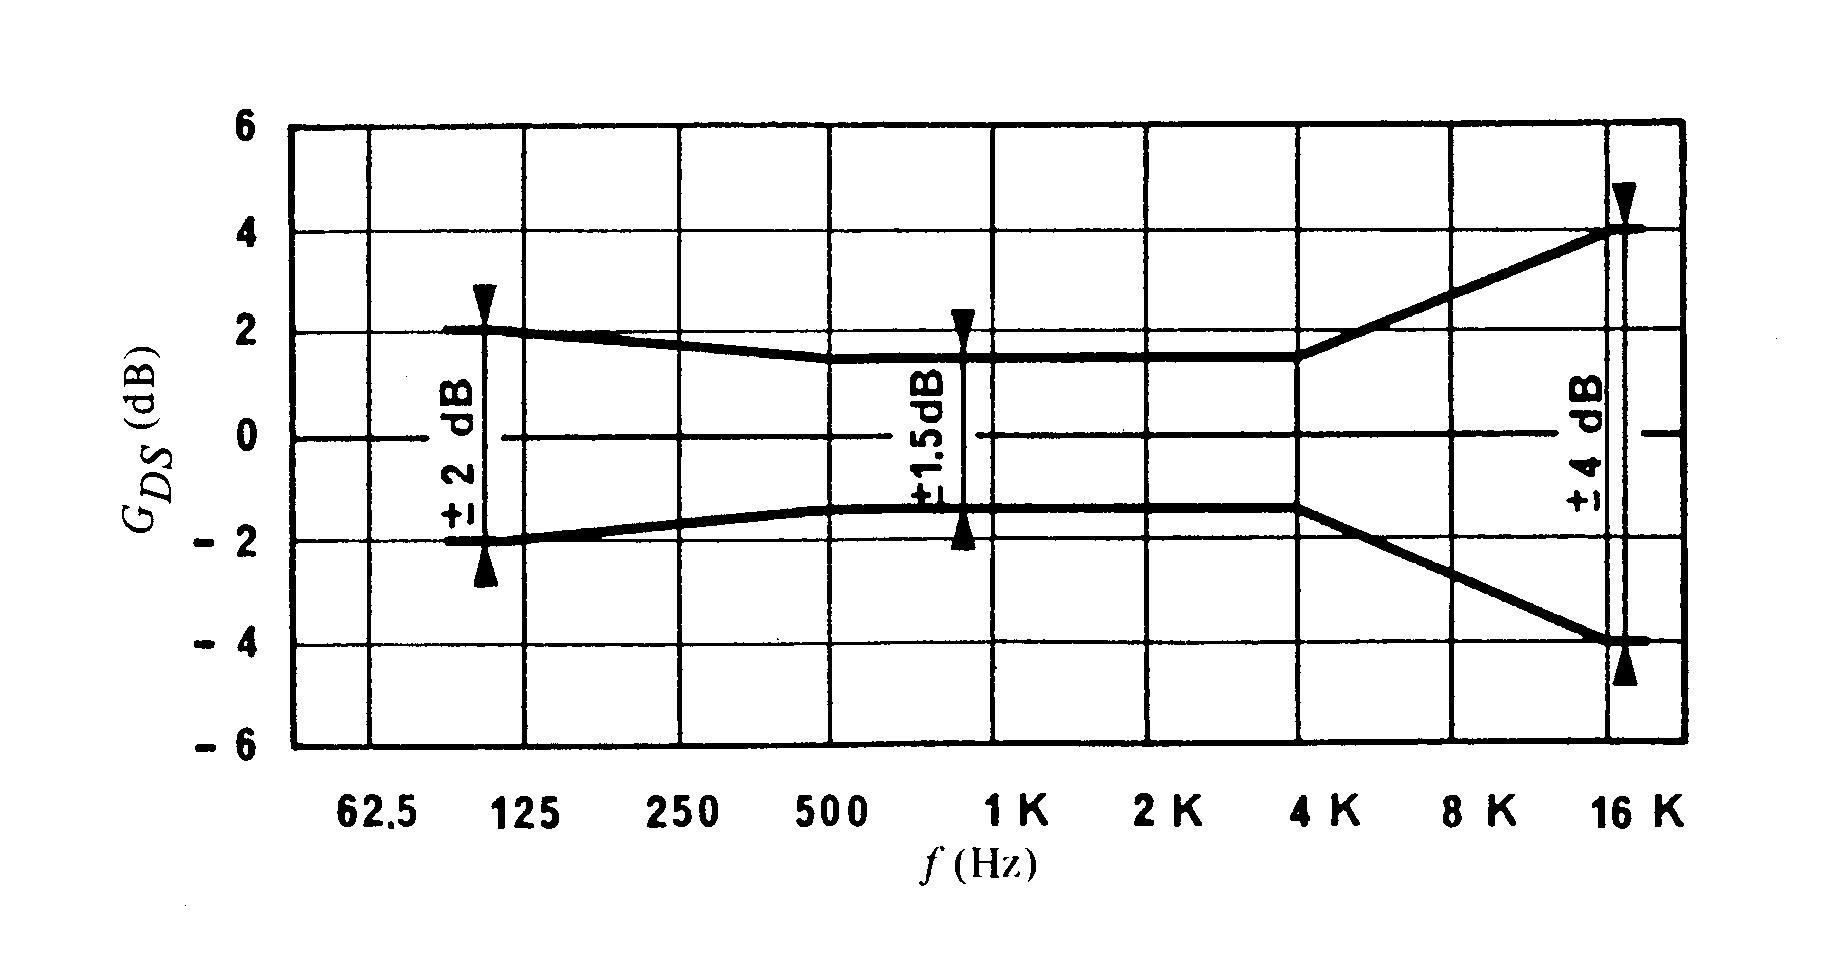
\includegraphics[width=.8\textwidth]{pic/headphones.png}
    \caption{Frekvenční toleranční maska studiových sluchátek z \cite{itur:708}}
    \label{pic:headphones}
\end{figure}


Samozřejmostí je, že všichni účastníci testu musí použít stejné poslechové zařízení.

\subsection{Statistická analýza}

Samotné provedení testu by bylo zbytečné bez provedení správné analýzy získaných dat. Podle knihy Základy statistiky \cite{book:statistika} se množina subjektů, na kterých je prováděno testování označuje jako \uv{výběr}. Cílem pokusu ovšem není zjistit \uv{výběrový průměr}, nýbrž aproximaci pro celou množinu potenciálních posluchačů. Zavádí se tedy pojem interval spolehlivosti ve kterém s nejvyšší pravděpodobností leží takzvaný \uv{populační průměr}. Jeho kalkulaci zahájíme výpočtem výběrového průměru $\bar{u}_{jk}$:

\begin{equation}
    \bar{u}_{jk}=\cfrac{1}{N}\sum_{i=1}^{N}u_{ijk}
\end{equation}

\noindent kde, $u_{ijk}$ značí hodnocení uživatele $i$ ve zkoušce $j$ testované metody zhoršení $k$ a $N$ odpovídá množství subjektů. Obdobným způsobem lze spočítat průměry $\overline{u}_j$ či například $\overline{u}_k$ \\

Doporučení \cite{itur:1534} říká, že výsledky mají být prezentovány na 95\% intervalu s krajními body:

\begin{equation}
    [\bar{u}_{jk} - \delta_{jk},\bar{u}_{jk} + \delta_{jk}]
\end{equation}

\noindent kde $\delta_{jk}$ je padesát procent šířky intervalu spolehlivosti daného vztahem: 

\begin{equation}
    \delta_{jk} = t_{0,05}\cfrac{\sigma_{jk}}{\sqrt{N}}
    \label{equation:inteval}
\end{equation}

\noindent a $t_{0,05}$ je hodnota odpovídající 95\% koeficientu spolehlivosti a stupni volnosti $N-1$, kterou lze najít ve statistických tabulkách. Směrodatná odchylka se poté spočítá podle:

\begin{equation}
    \sigma_{jk} =\sqrt{\sum_{i=1}^{N}\cfrac{(\bar{u}_{jk}-u_{ijk})^2}{N-1}}
\end{equation}
 
Vypočtením těchto hodnot zjistíme, že hodnota populačního průměru se nachází v intervalu spolehlivosti s pravděpodobností 95\%.



\subsection{Prezentace výsledků}

Zpracované výsledky by měly být prezentovány takovou formou, aby jim porozuměl jak laik tak expert v oboru. Na přehledném místě v textu by měl čtenář zprvu narazit na grafické zpracování s vyobrazeným intervalem spolehlivosti. To by mělo být doprovázené popisem toho co jednotlivé grafy vyjadřují nicméně není potřeba uvádět veškeré výpočty vedoucí k daným závěrům. Pokud je autor uvést chce, může je přiložit ve formě dodatku.
\smallskip

Opomenuto by tedy nemělo být následující: \begin{itemize}
    \item grafická reprezentace dosažených výsledků
    \item popis množiny subjektů: počet, průměrný věk..
    \item specifikace poslechového materiálu včetně důvodu pro výběr
    \item charakteristika poslechové místnosti včetně rozměrů, typy měničů, jejich umístění a konfigurace 
    \item popis metodiky testu
    \item způsob zpracování dat
    \
\end{itemize}